\documentclass{standalone}
\usepackage{pgfplots,amsmath}
\pgfplotsset{compat=1.18}
\usetikzlibrary{math,arrows.meta}

\begin{document}


\pgfplotsset{
  % height = 0.7\textwidth,
  width = 0.9\textwidth,
  scale only axis,
}

\newcommand{\vertLineFromPoint}[1]{
  \draw[dashed] 
	(#1) -- (#1|-{0,\pgfkeysvalueof{/pgfplots/ymin}})
}

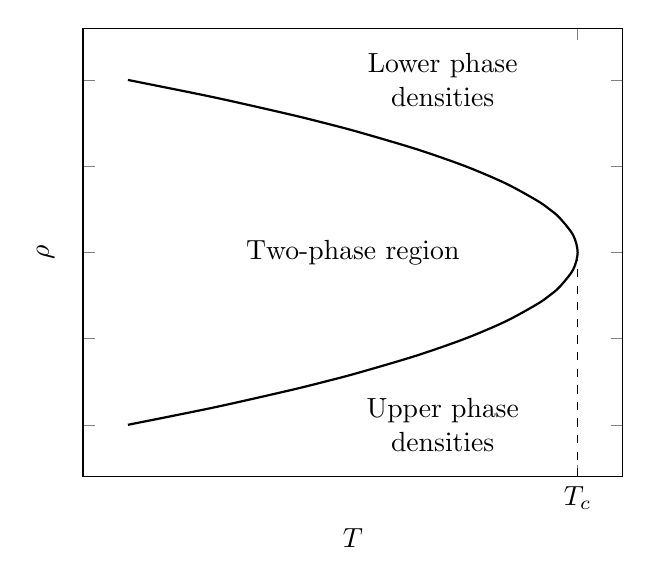
\begin{tikzpicture}
	\begin{axis}[
	clip=true,
	xtick={1},
	xticklabels={$T_c$},
	yticklabels=none,
	xlabel={$T$},
	ylabel={$\rho$},
	xmin=-0.1, xmax=1.1, 
	ymin=-1.3, ymax=1.3,
	]
	
	\addplot [mark=none,smooth,thick] coordinates {
				(0.0, 	-1.0)
				(0.19, 	-0.9)
				(0.36, 	-0.8)
				(0.4375, -0.75)
				(0.51, 	-0.7)
				(0.64,	-0.6)
				(0.75,	-0.5)
				(0.84, 	-0.4)
				(0.91, 	-0.3)
				(0.9375, -0.25)
				(0.96, 	-0.2)
				(.99,	-0.1)
				(1.0, 	0.0) 
				(.99,	0.1)
				(0.96, 	0.2)
				(0.9375, 0.25)
				(0.91, 	0.3)
				(0.84, 	0.4)
				(0.75,	0.5)
				(0.64,	0.6)
				(0.51, 	0.7)
				(0.4375, 0.75)
				(0.36, 	0.8)
				(0.19, 	0.9)
				(0, 	1)};	
	
	\draw [dashed] (1.0, 0.0) -- (1.0, -1.3);
	\node at (0.5,0) {Two-phase region};
	\node [align=center] at (0.7, -1.0) {Upper phase\\densities};
	\node [align=center] at (0.7, 1.0) {Lower phase\\densities};
	
	\end{axis}
\end{tikzpicture}

\end{document}
